
\documentclass[11pt]{exam} % https://www.ctan.org/pkg/exam?lang=en

\usepackage[lmargin=1.in,rmargin=1.in,tmargin=1.in,bmargin=1in]{geometry}
\usepackage{setspace}
\usepackage[pdftex]{graphicx}
\usepackage{titling}
\usepackage[
	pdfauthor={Brian Weinstein},
	pdftitle={Homework 1},
	bookmarks=true,
	colorlinks=true,
	linkcolor=blue,
	urlcolor=blue,
	citecolor=blue,
	pdftex,
	linktocpage=true
	]{hyperref}
\usepackage[textsize=tiny]{todonotes}
\usepackage{float}
\setlength\parindent{0pt}
\usepackage{lipsum}
\usepackage{amsmath}


\qformat{\textbf{Problem \thequestion: \thequestiontitle}\quad \hfill}


\pagestyle{headandfoot}
\runningheadrule
\firstpageheader{}{}{}
\runningheader{\theauthor}{\thetitle}{\thedate}
\firstpagefooter{}{\thepage}{}
\runningfooter{}{\thepage}{}


\usepackage{xcolor}
\usepackage{adjustbox}
\usepackage{verbatim}
\definecolor{shadecolor}{rgb}{.9, .9, .9}

\newenvironment{code}%
   {\par\noindent\adjustbox{margin=1ex,bgcolor=shadecolor,margin=0ex \medskipamount}\bgroup\minipage\linewidth\verbatim}%
   {\endverbatim\endminipage\egroup}

\newenvironment{codeSmall}%
   {\par\noindent\adjustbox{margin=1ex,bgcolor=shadecolor,margin=0ex \medskipamount}\bgroup\minipage\linewidth\verbatim\footnotesize}%
   {\endverbatim\endminipage\egroup}

\newcommand{\ramsey}{\href{http://www.statisticalsleuth.com/}{Ramsey }}


\begin{document}


\title{STAT S4201 001, Homework 1}
\author{Brian Weinstein (bmw2148)}
\date{Feb 3, 2016}
\maketitle


Code is attached here and also posted at \href{https://github.com/BrianWeinstein/advanced-data-analysis}{https://github.com/BrianWeinstein/advanced-data-analysis}. Where relevant, code snippets and output are are included in-line.

\begin{questions}


\titledquestion{\ramsey 1.17}

A subset of the 35 possible combinations, along with their sample averages and difference in sample averages is provided below:
\begin{code}
   a1 a2 a3 a4 b1 b2 b3 avg_a    avg_b    avg_diff
1  68 77 82 85 53 64 71 78.00 62.66667  15.3333333
2  68 77 82 53 85 64 71 70.00 73.33333  -3.3333333
3  68 77 82 64 85 53 71 72.75 69.66667   3.0833333
...
33 82 85 64 71 68 77 53 75.50 66.00000   9.5000000
34 82 53 64 71 68 77 85 67.50 76.66667  -9.1666667
35 85 53 64 71 68 77 82 68.25 75.66667  -7.4166667
\end{code}

The observed difference between sample averages is $15.333$, which, based on the 35 differences in the randomization distribution, corresponds to a two-sided p-value of $0.0867$.



\titledquestion{\ramsey 1.21}

\begin{parts}


\part A Trial of Wound Irrigation in the Initial Management of Open Fracture Wounds

\begin{subparts}
\setlength{\parindent}{1em}

\subpart \textit{Links:}

\footnotesize

Preview: \href{http://www.nejm.org/doi/full/10.1056/NEJMoa1508502}{www.nejm.org/doi/full/10.1056/NEJMoa1508502}

Full Article: \href{http://www.nejm.org.ezproxy.cul.columbia.edu/doi/full/10.1056/NEJMoa1508502\#t=article}{www.nejm.org.ezproxy.cul.columbia.edu/doi/full/10.1056/NEJMoa1508502\#t=article}

\normalsize


\subpart \textit{Summary of study design and conclusions:}

This study measured the effects of 6 different methods of wound irrigation and debridement for patients with open fractures. The researches measured ``castile soap versus normal saline irrigation delivered by means of high, low, or very low irrigation pressure.'' Patients who arrived at 41 participating clinics were randomly assigned to receive one of the six treatments.

As a measure of treatment efficacy, researchers recorded the number of participants that required at least one additional operation (to promote proper healing to treat wound infection) in the 12 months following the initial surgery.

The study found that irrigation pressure --- regardless of the choice between soap and saline --- didn't have a significant effect on reoperation rates (p-values between $0.53$ and $0.89$). The choice between soap and saline was significant (p-value $0.01$), with 14.8\% of the participants in the soap group requiring reoperation, compared to only 11.6\% of the participants in the saline group. The researchers concluded ``that very low pressure is an acceptable, low-cost alternative for the irrigation of open fractures,'' that ``saline was superior to castile soap,'' and that their study may have implications for patients worldwide.

\subpart \textit{Categorize the study according to Display 1.5.}

It isn't explicitly stated that participant selection was randomized, but it is strongly implied in both the ``Patients'' section and the eligibility criteria outlined in the \href{http://www.nejm.org.ezproxy.cul.columbia.edu/doi/suppl/10.1056/NEJMoa1508502/suppl_file/nejmoa1508502_appendix.pdf}{Supplementary Appendix (PDF)}. The allocation of participants to treatment group was randomized. The study therefore falls into the top-left group in Display 1.5.

\subpart \textit{Determine whether inferential statements are limited to or go beyond the scope allowed in Display 1.5.}

The researchers' conclusions make both causal inferences and inferences to the population, both of which are allowed by the study's placement in Display 1.5.

\end{subparts}



\part A Randomized, Controlled Trial of an Aerosolized Vaccine against Measles


\begin{subparts}
\setlength{\parindent}{1em}

\subpart \textit{Links:}

\footnotesize

Preview: \href{http://www.nejm.org/doi/full/10.1056/NEJMoa1407417}{www.nejm.org/doi/full/10.1056/NEJMoa1407417}

Full Article: \href{http://www.nejm.org.ezproxy.cul.columbia.edu/doi/full/10.1056/NEJMoa1407417\#t=article}{www.nejm.org.ezproxy.cul.columbia.edu/doi/full/10.1056/NEJMoa1407417\#t=article}

\normalsize

\subpart \textit{Summary of study design and conclusions:}

This study measured the effect of a measles vaccine delivered via aerosol inhalation vs subcutaneous injection. Children in Pune, India between the ages of 9.0 and 11.9 months who were eligible to receive the vaccine (according to WHO criteria) were randomly selected to participate in the experiment, and were randomly assigned in a 1:1 ratio to one of the treatment groups.

Researchers were testing the hypothesis that the aerosol inhalation was not inferior to the subutaneous injection. As a measure of treatment efficacy, researchers tested if (1) the participant was seropositive (had antibodies against measles) 91 days after vaccination, and (2) the participant had any adverse effects in the 0--90 days after vaccination.

On day 91, 85.4\% of the aerosol group (95\% CI, 82.5 to 88.0) was seropositive, compared to 94.6\% of the subcutaneous group (95\% CI, 92.7 to 96.1); a difference of −9.2 percentage points (95\% CI, −12.2 to −6.3). The researchers found that, at the pre-specified 5 percentage-point margin, ``the aerosolized vaccine was inferior to the subcutaneous vaccine with respect to the rate of seropositivity.'' There were no serious adverse events attributable to measles vaccination in either group. The study concluded that the aerosolized vaccine was inferior to the subcutaneous injection when measuring ``seropositivity at 91 days in children who were 9.0 to 11.9 months of age.''


\subpart \textit{Categorize the study according to Display 1.5.}

Since both the participant selection and group allocation were randomized, the study falls into the top-left group in Display 1.5.

\subpart \textit{Determine whether inferential statements are limited to or go beyond the scope allowed in Display 1.5.}

The researchers' conclusion makes both a causal inference and an inference to the population, both of which are allowed by the study's placement in Display 1.5.

\end{subparts}




\end{parts}




\titledquestion{\ramsey 1.25 (b)}

A boxplot of zinc concentrations in the blood for two groups of rats is shown in Figure \ref{fig:3}.
 
\begin{code}
# load data
ratData <- Sleuth3::ex0125

# create boxplots
ggplot(ratData, aes(x=Group, y=Zinc)) +
  geom_boxplot() + 
  ylab("Zinc concentration (mg/ml)")
\end{code}

\begin{figure}[h!]
	\centering
	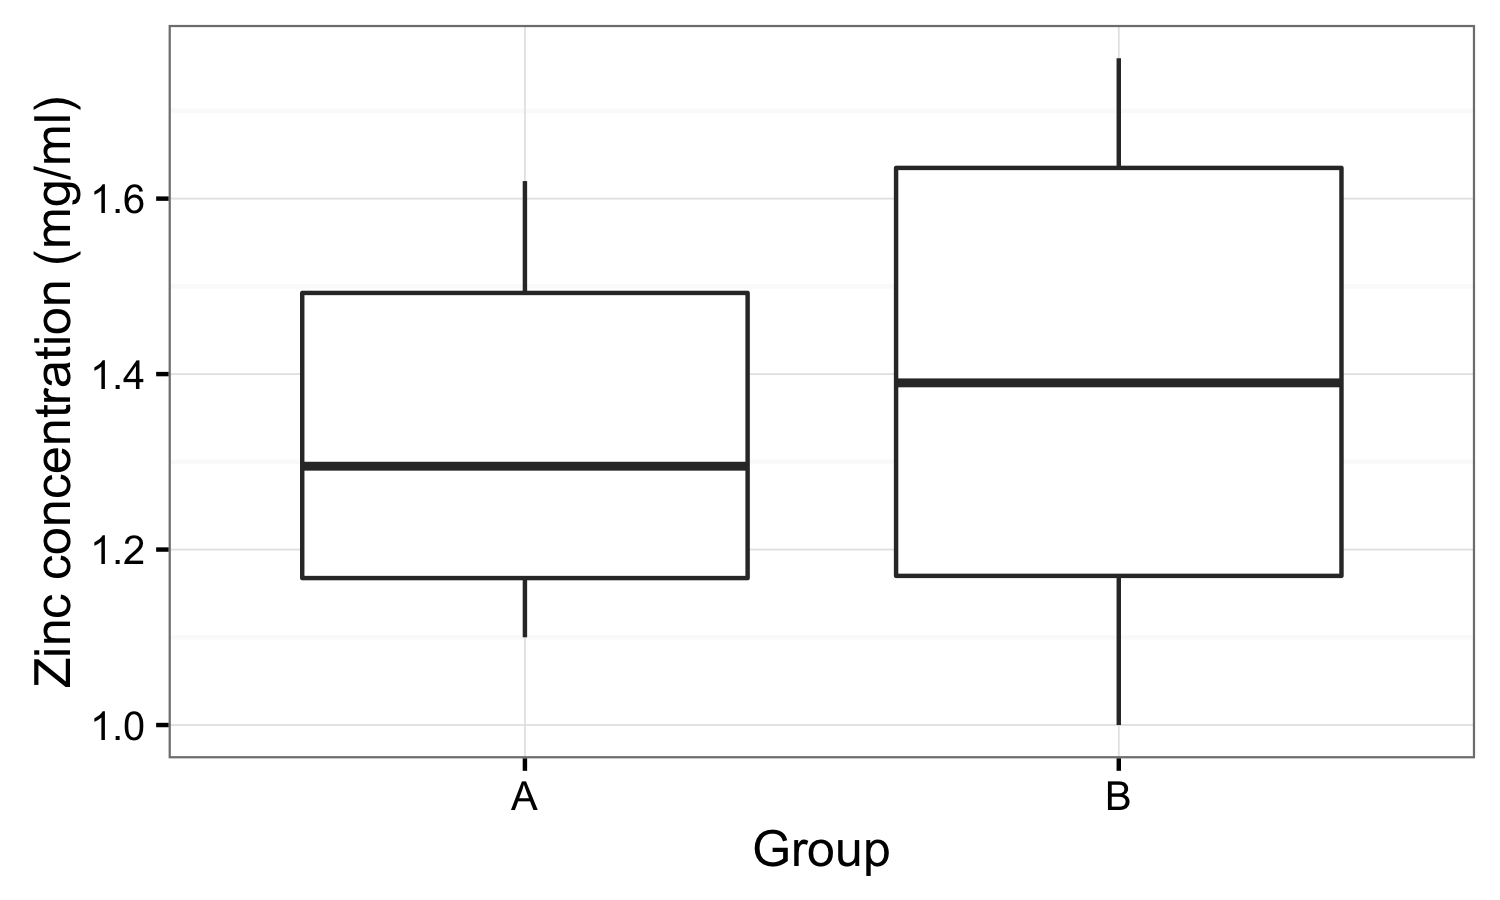
\includegraphics[width=5in]{3.png}
	\caption{Zinc concentrations (in mg/ml) in the blood for two groups of rats. Group A received a calcium supplement and Group B did not.}
	\label{fig:3}
\end{figure}




\titledquestion{Use the data from Problem 3 to answer the following questions.}

See attached code.

\begin{parts}

\part \textit{Set up the null and alternative hypotheses to address the research question described.}

\begin{itemize}
\item Test statistic $t=\bar{A}-\bar{B}$, where $\bar{A}$ and $\bar{B}$ are the average Zinc concentrations in the rats of group A and B, respectively.
\item Null hypothesis: $t=0$
\item Alternative hypothesis: $t\neq0$
\end{itemize}


\part \textit{Use 1,000 simulations to perform a randomization test for testing the hypothesis in (a). What is your p-value?}

The observed difference between sample averages is $-0.07755$, which, based on the 1,000 simulations in the randomization distribution, corresponds to a two-sided p-value of $0.261$.

\part \textit{Draw the reference distribution of your test statistic based on 1,000 simulations.}

See Figure \ref{fig:4c}.

\begin{figure}[h!]
	\centering
	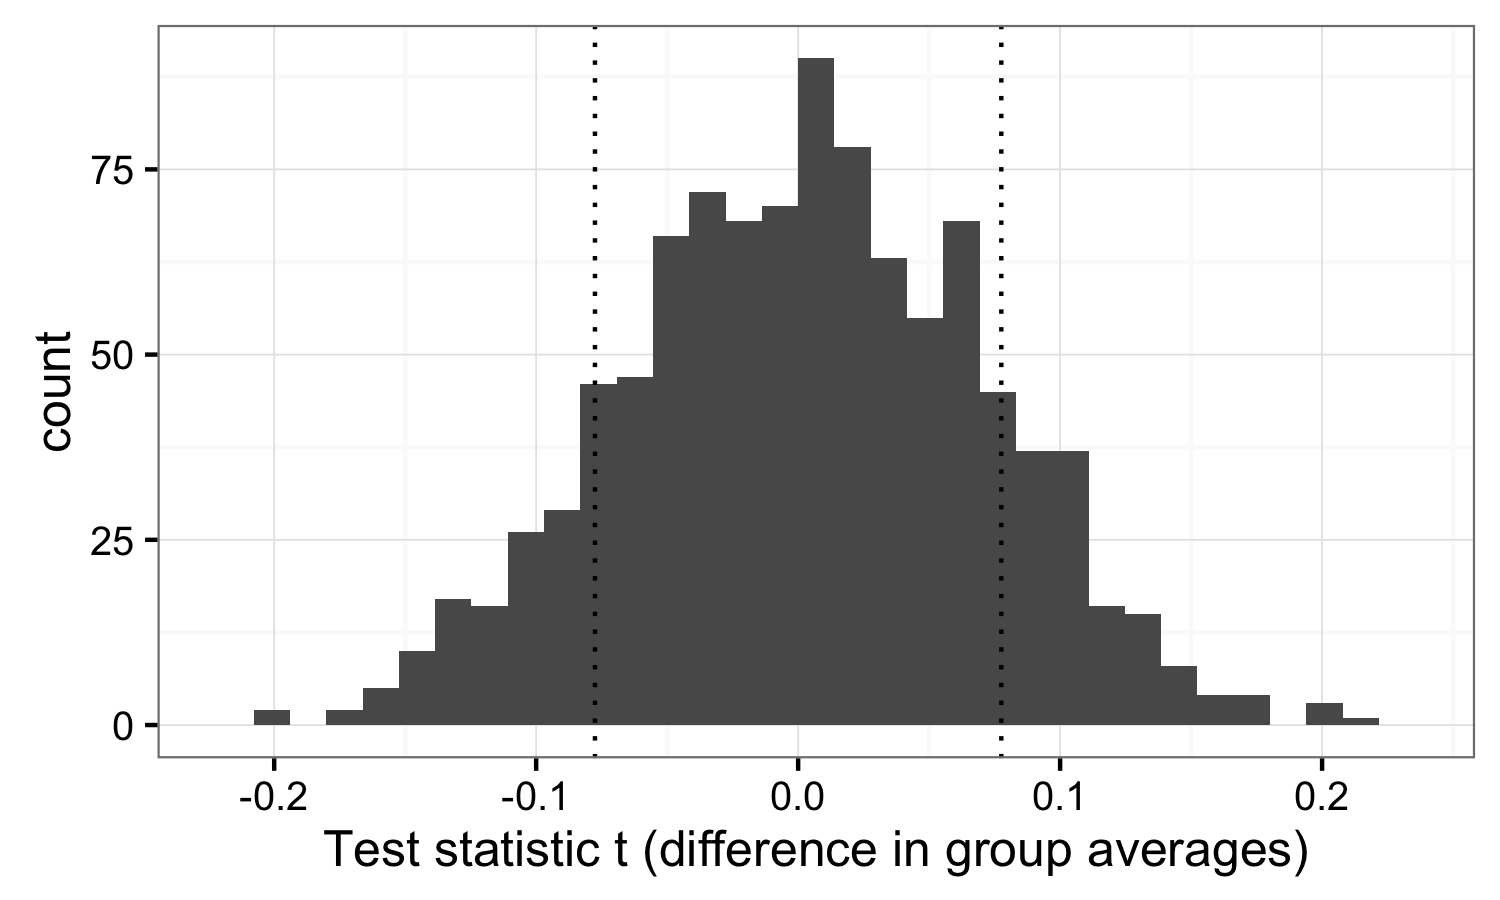
\includegraphics[width=5in]{4c.png}
	\caption{Reference distribution of $t$, based on 1,000 simulations.}
	\label{fig:4c}
\end{figure}


\part \textit{Write a brief summary of your findings and possible recommendations for the researchers.}

The available data does not provide conclusive evidence that the calcium supplement given to group A, but not to group B, had an effect in blood Zinc concentrations. The p-value, $0.261$, associated with the test statistic indicates that there isn't enough evidence to conclusively reject the null hypothesis.



\end{parts}




\titledquestion{\ramsey 2.12}

\begin{align*}
& \mu_1 = \text{average birthweight of babies from mothers who used marijuana} \\
& \mu_2 = \text{average birthweight of babies from mothers who did not use marijuana} \\
& \mu_2 - \mu_1 = 280 \text{ grams} \\
& \text{SE}\left(  \mu_2 - \mu_1  \right) = 46.66 \text{ grams, with d.f.} = 1095
\end{align*}


\begin{parts}

\part A 95\% confidence interval for $\mu_2 - \mu_1$ is from $188.4469$ to $371.5531$.

\begin{codeSmall}
> # Define a fn to calcuate a conf interval for a given mean, std error, df, and conf level
> MakeConfidenceInterval <- function(mean, se, df, confLevel){
+   sigLevel <- 1 - confLevel
+   error <- qt(p=1-(sigLevel/2), df=df) * se
+   lowerBound <- mean - error
+   upperBound <- mean + error
+   confidenceInterval <- c(lowerBound, upperBound)
+   return(confidenceInterval)
+ }
> 
> # define variables for this problem
> mean_value <- 280
> std_err <- 46.66
> df_value <- 1095
> 
> MakeConfidenceInterval(mean=mean_value, se=std_err, df=df_value, confLevel=0.95)
[1] 188.4469 371.5531
\end{codeSmall}



\part A 90\% confidence interval for $\mu_2 - \mu_1$ is from $203.1861$ to $356.8139$.

\begin{codeSmall}
> MakeConfidenceInterval(mean=mean_value, se=std_err, df=df_value, confLevel=0.90)
[1] 203.1861 356.8139
\end{codeSmall}



\part A two-sided p-value for a test of the hypothesis that $\mu_2 - \mu_1 = 0$ is minuscule, at $2.7 \times 10^{-9}$.

\begin{codeSmall}
> # t-statistic: (mean - hypothesized_mean) / se, for hypothesized_mean=0
> t_stat <- (mean_value - 0) / std_err
> t_stat
[1] 6.000857
> 
> # two-sided p-value for this t statistic
> 2 * pt(q=(-1 * abs(t_stat)), df=df_value)
[1] 2.664672e-09
\end{codeSmall}


\end{parts}


\titledquestion{\ramsey 2.14}

Using the \texttt{t.test} R function,
\begin{code}
fishOilData <- Sleuth3::ex0112
t.test(formula=BP~Diet, data=fishOilData,
       var.equal=TRUE, conf.level=0.95)
\end{code}

a 95\% confidence interval for $\mu_2 - \mu_1$ is given by $2.225 < \mu_2 - \mu_1 < 13.203$.

Since we care about a one-sided effect (that the fish oil diet resulted in greater reduction of blood pressure), we could alternatively look at a one-sided 95\% confidence ``interval'':
\begin{code}
t.test(formula=BP~Diet, data=fishOilData,
       var.equal=TRUE, conf.level=0.95,
       alternative="greater")
\end{code}

to find $3.224 < \mu_2 - \mu_1 < \infty$.

The one-sided p-value is $0.004931$.



\titledquestion{\ramsey 2.16}

Using the \texttt{t.test} R function on the "Motivation and Creativity" case study data from Section 1.1.1.,
\begin{code}
> # load data
> creativityData <- Sleuth3::case0101
> 
> # reorder Treatment factor levels to be consistent with book's analysis
> creativityData$Treatment <- relevel(creativityData$Treatment, "Intrinsic")
> 
> # compute t-test
> t.test(formula=Score~Treatment, data=creativityData,
+        var.equal=TRUE, conf.level=0.95)

	Two Sample t-test

data:  Score by Treatment
t = 2.9259, df = 45, p-value = 0.005366
alternative hypothesis: true difference in means is not equal to 0
95 percent confidence interval:
 1.291432 6.996973
sample estimates:
mean in group Intrinsic mean in group Extrinsic 
               19.88333                15.73913 
\end{code}

we find a two-sided p-value of $0.0054$, and a treatment effect of $19.88-15.74=4.14$ with a 95\% confidence interval of $1.29$ to $7.00$ points.

These values are consistent with those stated in Section 1.1.1 (p-value $0.005$; treatment effect $4.1$ points with 95\% confidence interval from $1.3$ to $7.0$ points).


\titledquestion{\ramsey 2.23}

There's very little evidence to suggest that the percentage change in traffic fatalities was greater in states that increased their speed limits. See Figure \ref{fig:8} for a boxplot showing the distribution of percent changes for the states that increased their speed limits (Inc) and the states that retained their speed limits (Ret).

\begin{figure}[h!]
	\centering
	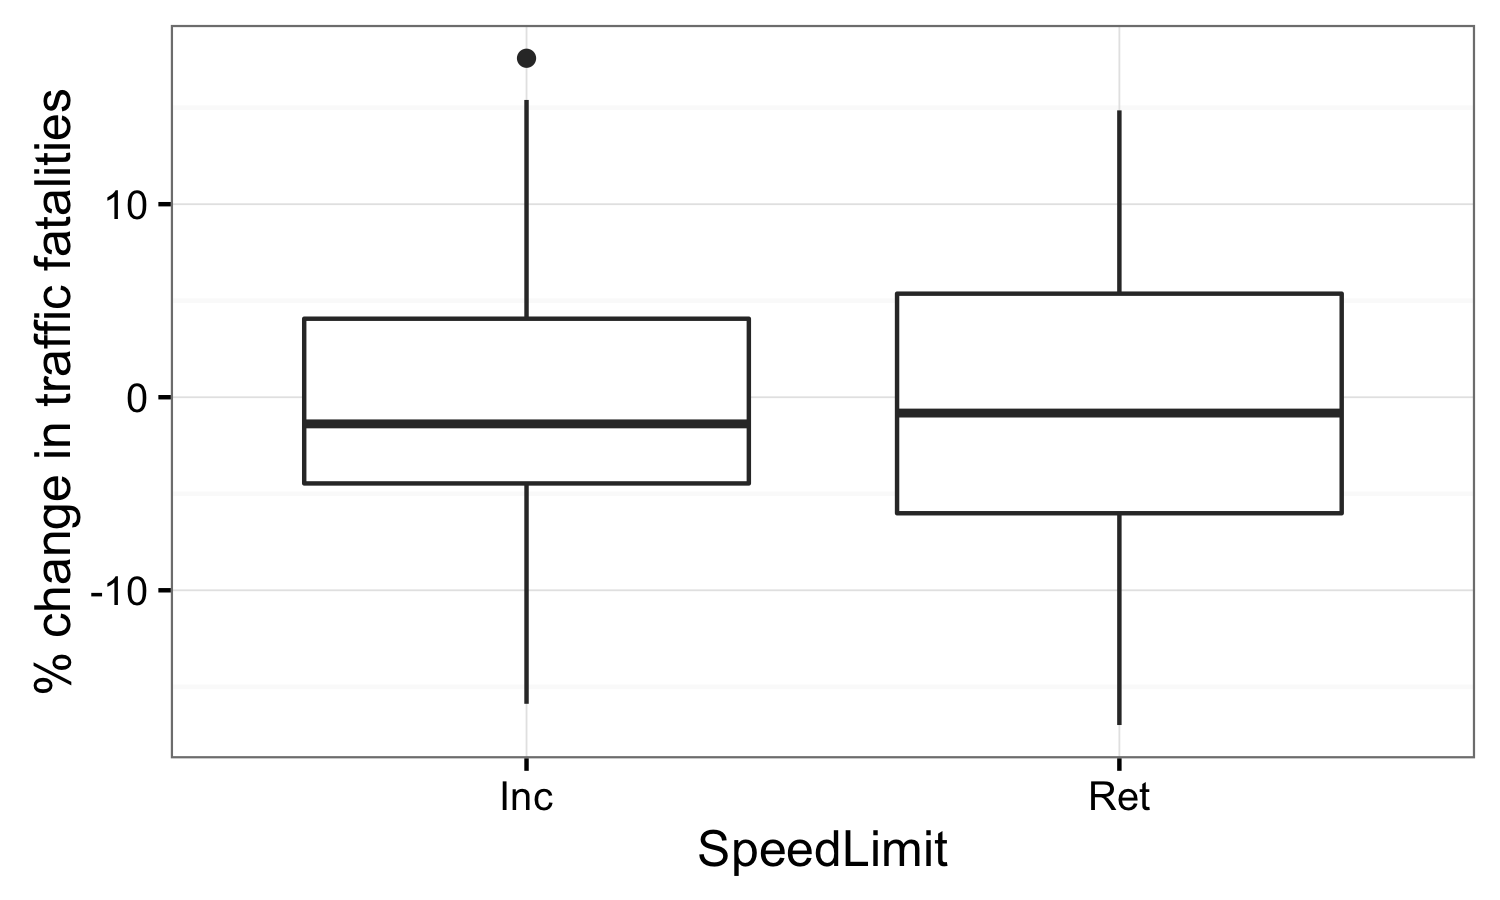
\includegraphics[width=5in]{8.png}
	\caption{Percent changes for the states that increased their speed limits (Inc) and the states that retained their speed limits (Ret). The outlier in the Inc group is from Texas, with a 17.45\% increase in fatalities from 1995 to 1996.}
	\label{fig:8}
\end{figure}


Performing the t-test on this data generates a one-sided p-value of $0.43495$ and a treatment effect of $0.39428$ in units of percent change (95\% CI from $-4.417753$ to $5.206305$). The treatment effect is mostly driven by three states with extremely large percent increases: Texas (the outlier in Figure \ref{fig:8}), Oklahoma, and Wyoming.

The high p-value indicates that there is nearly no evidence to reject the null hypothesis, which states that the difference in means $\mu_{Inc} - \mu_{Ret}$ is positive.


\end{questions}

% \listoftodos

\end{document}
